% Options for packages loaded elsewhere
\PassOptionsToPackage{unicode}{hyperref}
\PassOptionsToPackage{hyphens}{url}
%
\documentclass[
  12pt,
]{article}
\usepackage{amsmath,amssymb}
\usepackage{lmodern}
\usepackage{ifxetex,ifluatex}
\ifnum 0\ifxetex 1\fi\ifluatex 1\fi=0 % if pdftex
  \usepackage[T1]{fontenc}
  \usepackage[utf8]{inputenc}
  \usepackage{textcomp} % provide euro and other symbols
\else % if luatex or xetex
  \usepackage{unicode-math}
  \defaultfontfeatures{Scale=MatchLowercase}
  \defaultfontfeatures[\rmfamily]{Ligatures=TeX,Scale=1}
\fi
% Use upquote if available, for straight quotes in verbatim environments
\IfFileExists{upquote.sty}{\usepackage{upquote}}{}
\IfFileExists{microtype.sty}{% use microtype if available
  \usepackage[]{microtype}
  \UseMicrotypeSet[protrusion]{basicmath} % disable protrusion for tt fonts
}{}
\makeatletter
\@ifundefined{KOMAClassName}{% if non-KOMA class
  \IfFileExists{parskip.sty}{%
    \usepackage{parskip}
  }{% else
    \setlength{\parindent}{0pt}
    \setlength{\parskip}{6pt plus 2pt minus 1pt}}
}{% if KOMA class
  \KOMAoptions{parskip=half}}
\makeatother
\usepackage{xcolor}
\IfFileExists{xurl.sty}{\usepackage{xurl}}{} % add URL line breaks if available
\IfFileExists{bookmark.sty}{\usepackage{bookmark}}{\usepackage{hyperref}}
\hypersetup{
  pdftitle={Assignment tariff plan non-life insurance},
  hidelinks,
  pdfcreator={LaTeX via pandoc}}
\urlstyle{same} % disable monospaced font for URLs
\usepackage[margin = 1in]{geometry}
\usepackage{graphicx}
\makeatletter
\def\maxwidth{\ifdim\Gin@nat@width>\linewidth\linewidth\else\Gin@nat@width\fi}
\def\maxheight{\ifdim\Gin@nat@height>\textheight\textheight\else\Gin@nat@height\fi}
\makeatother
% Scale images if necessary, so that they will not overflow the page
% margins by default, and it is still possible to overwrite the defaults
% using explicit options in \includegraphics[width, height, ...]{}
\setkeys{Gin}{width=\maxwidth,height=\maxheight,keepaspectratio}
% Set default figure placement to htbp
\makeatletter
\def\fps@figure{htbp}
\makeatother
\setlength{\emergencystretch}{3em} % prevent overfull lines
\providecommand{\tightlist}{%
  \setlength{\itemsep}{0pt}\setlength{\parskip}{0pt}}
\setcounter{secnumdepth}{5}
\ifluatex
  \usepackage{selnolig}  % disable illegal ligatures
\fi
\usepackage[]{natbib}
\bibliographystyle{plainnat}

\title{Assignment tariff plan non-life insurance}
\author{}
\date{\vspace{-2.5em}11/05/2021}

\begin{document}
\maketitle

\tableofcontents
\pagebreak

\hypertarget{introduction}{%
\section{Introduction}\label{introduction}}

\hypertarget{binning-of-spatial-data}{%
\subsection{Binning of Spatial Data}\label{binning-of-spatial-data}}

Spatial data was represented as a pair of coordinates in the dataset.
These correspond to the center of each of the Belgian cities. In this
way they could be linked to the postal codes, which is a known variable
for each policy holder in the dataset. This allows us to make
predictions of the claim frequency and claim severity based on the city
that a policy holder lives in. Then based on these predictions the
postal codes can be binned in an optimal number of factors.

To start, a model to estimate the predicted frequency and severity needs
to be constructed. A Generalized Additive Model will be used for this
purpose. A base model to model spatial data is
\(y ~ s(long, lat, bs=”tp”)\). From here on, there will be differences
between frequency and severity because they will each have their own
optimal GAM-model, based on different dataset. Frequency used all
observations, while the severity dataset makes abstraction of policy
holders that did not file a claim in the observation period. Note that a
smoother was used for longitude and latitude coordinates, which makes us
able to see regions with higher expected claim frequency or expected
claim amount. If only postal codes were used, these regional effect
would not be visible and all cities would be seen as independent of
their location with respect to each other.

For frequency, we use a Poisson-family with a log-link function which is
a logical choice when modeling claim frequency in an insurance context.
Also, the exposure needs to be added as an offset due to a not all
policy holders being covered for a full year and due to modifications
(eg. people that move change their postal code, people that buy a more
powerfull car). The spatial model is then extended with different other
variates. By comparing the log-likelihood and the Akaiki Information
Criterion (AIC) of different GAM-models, the most optimal GAM for
frequency data was found:\$ freq \textasciitilde{} s(ageph) +
s(long,lat) + power + cover + fleet + split + fuel + sexph + agecar\$.
Also, this model was constructed with a Restricted Maximum Likelihood
(REML), while still applying the offset and the same family and
linkfunction.

\hypertarget{binning-of-age-variable}{%
\subsection{Binning of Age Variable}\label{binning-of-age-variable}}

In the dataset used to price our insurance products, age is recorded as
a continuous variable with ages ranging from 17 to 95 years old. To
optimally use a GLM, it is advised to use only categorical variables,
and thus age is best converted to an ordered factor variable. Again,
because there is a difference in the used dataset for frequency and
severity modelling, the breakpoints may differ.

For claim frequency, the GAM-model used for the binning of spatial data
was reused, but with the binned version of the spatial data as a
replacement for its continuous counterpart. All other aspects identical.
So the used formula is:
\(freq ~ s(ageph) + geo + power + cover + fleet + split + fuel + sexph + agecar\),
with `geo' being the binned spatial variable. By predicting the claim
frequency and constructing a new dataset (GAM\_data) where the
observations are counted per value of age. This is possible because
`age' is not really a continuous variable, it can only take positive
integer values. In this dataset, the coefficient of the smoother of
`age' is also included. Based on GAM\_data, the evtree( )-function in R
can be used to construct a regression tree based on an evolutionary
algorithm and with the counts per age as weights. In this function, it
is usefull to include an evtree.control( ), which controls the
complexity of the constructed tree. 4 Parameters were used for this
goal, with the first being the alpha, which was set to 100. Also, the
maximum depth of the tree was set to 5 to control the size of the tree.
The two last control parameters were set to control the choice of
splitting or not. `minbucket' Sets the minimum sum of weights in a
terminal note, here set to 5\% of the total weights in the training set.
`minsplit' Determines the needed minimum sum of weights in a node to
consider a split, here set to 10\% of the total weights in the training
set.

The constructed tree yields the following breakpoints: 17, 26, 29, 32,
35, 38, 51, 55, 59, 63, 73, 95, which makes for 11 bins. This tree can
also be graphed:

Clearly, the differences in expected claim frequency per bin can be seen
in the boxplots below each bin in the tree. Policy holders younger than
26yo have a higher expected claim frequency compared to for example a
55yo policy holder. The binned variable is added to the original dataset
under `agephGR'.

\hypertarget{exploratory-analysis}{%
\subsection{Exploratory Analysis}\label{exploratory-analysis}}

\hypertarget{frequency}{%
\subsubsection{Frequency}\label{frequency}}

\hypertarget{severity}{%
\subsubsection{Severity}\label{severity}}

we started the exploratory analysis on the severity by looking at the
density of logarithmic claim amounts. From the density we can clearly
see that the data is not following any well-behaved distribution and we
thus opted for using the gamma distributions as this distribution is
more versatile than the log-normal. From the graph we can also deduct
that there are a lot of outliers, which is expected for claim amounts as
they tend to deviate from the mean. Next, the mean, variance, skewness
and kurtosis are 1866.57, 19338.67, 78.84, 7701.894 respectively. This
also indicated a lot of deviation on the positive side and frequent
outliers as the kurtosis is substantial. This result also emphasize the
conclusion we made from the graph. The following figure is a
representation of the relative claim amounts per county where we
subdivide the claim amounts per county according to the following
quantiles: 0.2, 0.8 , 0.9, 0.95 and 0.99 . From the map of Belgium we
can say that most of the claim amounts occur in the cities like
Brussels, Antwerp and Liege. Although, there are some counties where the
claim amount is also a sizable amount, for example in the Hainaut
Province. This probably indicates that some outliers might be located in
these regions.

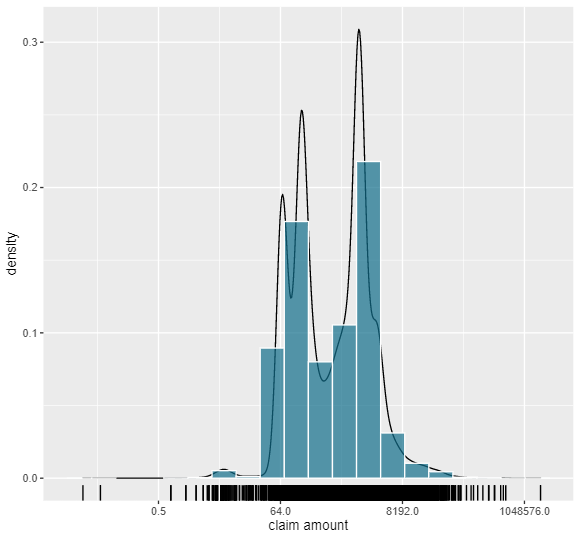
\includegraphics[width=0.5\textwidth,height=\textheight]{Severity_Analysis/plots/exploratory/density.png}
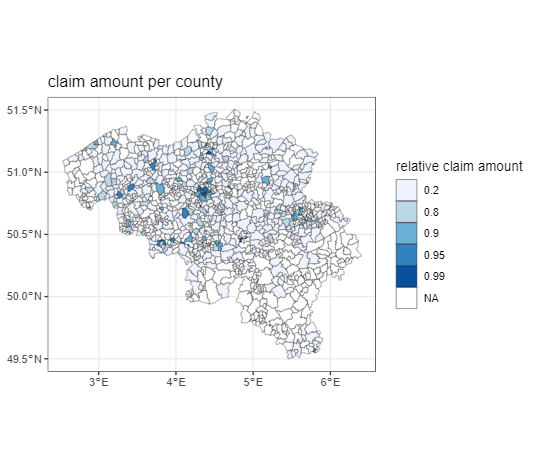
\includegraphics[width=0.5\textwidth,height=\textheight]{Severity_Analysis/plots/exploratory/county.png}

Now that the claim amounts have been plotted according to the postal
codes, we can subsequently plot the claim amounts based on the other
independent variables. Here it is clearly visible that there are some
variables which could be redundant and thus have less explanatory power
than the others. For example the variables use, fleet and sport car are
highly homogeneous and likely not able to explain a lot of the variation
in our depended variable. Also, the variables sex, fuel and power do not
have a visible impact on claim amounts. On the other hand, the variables
age of the car, cover, split and the binned version of policy holders
age create a detectable change in the claim amounts and will thus be
more likely to explain our depend variable. Note, that the outliers are
primarly located in cars with six to ten years of age from males between
38 and 51 having a one time split of the premium with a MTPL cover. But
we also need to be carefull of this explaination as this is also the
largest subgroup in the population and might as well just posses these
outliers in proportion.

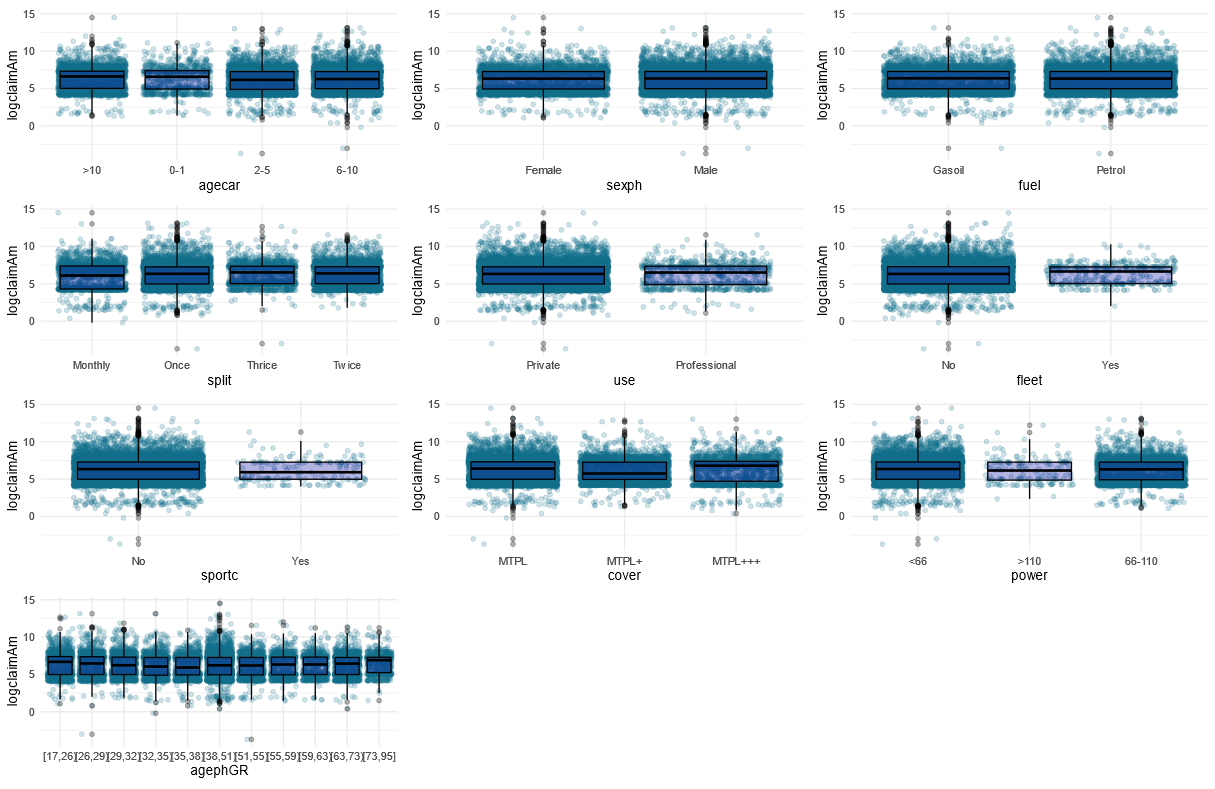
\includegraphics[width=1\textwidth,height=\textheight]{Severity_Analysis/plots/exploratory/barplots.png}

\hypertarget{interaction-effects}{%
\subsection{Interaction Effects}\label{interaction-effects}}

Now that we have looked at the independent variables with respect to the
dependent variable we want to have a closer look at the interaction
effects between the independent variables. To do this we follow the
paper of \citet{chavent2011clustofvar}. \citet{chavent2011clustofvar}
measured the homogeneity between variables by looking at the squared
Pearson correlation \(r^2\) and the correlation ratio \(\eta^2\) between
the variables. They defined the homogeneity of a cluster of variables
\(C_k\) as:

\[ H(C_k) = \sum_{x_j \in C_k} r^2_{x_j,y_k} + \sum_{z_j \in  C_k} \eta_{y_k|z_j} = \lambda^k\]
Where \(x_j\) are the quantitative variables, \(z_j\) are the
qualitative variables and \(y_k\) is the first principle component (PCA)
of the cluster ( or the synthetic variable of the cluster). Then,
\citet{chavent2011clustofvar} deviced an algorithm which chooses the
partition which maximizes the homogeneity of the cluster. This is done
in nested approach giving us the dendogram below.

The interaction between the variables is shown in the dendogram.
Clearly, `sportc' and `power' are closely linked, which can perfectly be
explained by the logic that sportscars mostly have a more powerfull
engine. Also the stronger correlation between the age of the car and the
type of cover can be explained: most newer cars have an MTPL-coverage,
while older cars tend to go for MTPL+ or MTPL+++. Next, the link between
`use' and `fleet' can be explained by the fact that most
professional-use cars are company cars which are part of a fleet.
Lastly, an interaction between the age of the policyholder and the
payment method (`split') is studied based on the logic that younger
people prefer to split their premium payments due to them having less
money to spend compared to older people. Although, looking at the graph,
this relation is not observable in the data.

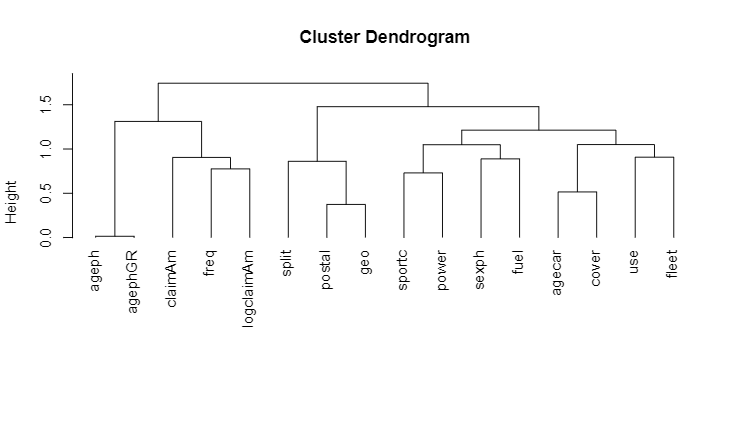
\includegraphics[width=0.75\textwidth,height=\textheight]{Severity_Analysis/plots/exploratory/dendogram.png}

\hypertarget{model-building}{%
\section{Model Building}\label{model-building}}

\hypertarget{frequency-1}{%
\subsection{Frequency}\label{frequency-1}}

Frequency analysis will be done using two models. On the one hand a
Generalized Linear Model and on the other hand a Gradient Boosting
Machine. Both will be compared whether they have sufficient predictive
power, given their complexity. The final model will be chosen based on
the higher accuracy on unseen data, while maintaining as simple as
possible. A GLM is much simpler compared to a GBM, but is a lot less
flexible.

\hypertarget{generalized-linear-model-glm}{%
\subsubsection{Generalized Linear Model
(GLM)}\label{generalized-linear-model-glm}}

A GLM was chosen because it is one of the most interpretable models of
all possible models, which is very important when explainability is an
important factor as it is in the insurance industry. A simple model is
easy to explain to the legislator and other stakeholders who may not be
an expert in this field. As already mentioned, a GLM is not the most
flexible model of the bunch. It requires linear relations and is
preferably modelled with categorical independent variables. Because of
this the spatial variable and the variable of the age of the
policyholder were binned into two factor variables, as discussed
earlier.

To find the optimal GLM, the simplest possible model was used as a
starting point: freq \textasciitilde{} 1. Because Poisson is a good
distribution for frequency data, the Poisson family was used when
constructing GLM's with the logarithm of exposure as an offset to
correct for non-full years of coverage. On this base case, other
variables were added one by one and their drop in deviance was compared.
The added variable which constituted the biggest drop in deviance, given
this drop was significant compared to a Chisq. critical value, was kept.
Once all singular variables were exhausted, interaction terms were
considered, limited to two-way interactions. Not all possible
interactions were tested, but only the logical ones and the ones based
on a Dendogram (see Interaction Effects).

In the added Excel-file (tab `GLM'), the reader can follow and compare
all the added variables in each step. As an example, the first box is
added which is used to find the first variable to add to the model. The
first line is the base case (glm0), respresented by the formula freq
\textasciitilde{} 1, with a deviance of 72.239 and 130.926 degrees of
freedom. Each line in the second box represents a different added
variable. Every model has its own deviance and degrees of freedom. By
comparing these with the base case, the model with the biggest drop in
deviance can be selected. In this case adding `agephGR' gives the
biggest significant drop in deviance, while `use' gives the smallest.
The p-values of each added variable were calculated using the
Chi-squared distribution. Following these findings, the model to proceed
with is \(freq ~ 1 + agephGR\), which will be used as the new base case
for adding a second variable.

Applying this method repeatedly it can be shown that the most optimal
GLM, given the observed training dataset is:

As a last check whether the aded variables are indeed significant and
meaningful, the optimal GLM is compared to the initial base case (glm0).
The output below (anova with Chi-squared test) shows a drop in deviance
of 2163,7, a difference of 37 degrees of freedom which lead to a p-value
small enough to make almost-certain conclusions (***).
\((add output of anova(glm0,glm_opt))\)

\hypertarget{gradient-boosting-machine-gbm}{%
\subsubsection{Gradient Boosting MAchine
(GBM)}\label{gradient-boosting-machine-gbm}}

A second approach to modelling frequency data, was by applying a
Gradient Boosting Machine. Gradient Boosting is a machine learning
technique for regression and classification problems to build a
predictive model as an ensemble of weak predictive models. It builds
sequential models, in contrast to random forest which builds in
parallel, and optimizes an arbitrary differentiable loss function
(SOURCE). This differentiable loss function is the Poisson deviance for
this application, due to it being used widely when modelling claim
frequency. In short, GBM combines weak learners into a single strong
learner in an iterative way. By doing this, the model becomes rather
flexibel compared to simpler models as a GLM. But this approach has a
much lower interpretability and explainability. Just imagine having to
provide every tree in the sequence to explain why a certain prediction
comes about. Obviously this is much harder than just offering a Least
Squares model that can be interpreted by almost anyone with basic
statistical knowledge.

Gradient Boosting has two tuning paramters which need to be optimized.
On the one hand the number of sequential trees (n.trees, T) needs to be
determined, and on the other hand the interaction depth
(interaction.depth, d) needs to be determined. T is rather self
explanatory in the sense that more trees make for a complexer, but a
more flexible model. The interaction depth might need some added
explanation. When d is 1, an additive model is made. When d is 2, the
algorithm allows up to two-way interaction. Also, note that when d
increases, the complexity of the model will also increase.

Besides tuning parameters, also two hyperparameters need a value
assigned to them. Firstly a shrinkage paramter (0\textless λ\textless1)
needs to be assigned, which determines the learning rate or step-size
reduction of each iterative tree. Assigning a higher value to this
parameter will result in better performance, but will also increase the
number of trees and thus increase the computational time. For this
application, a value of 0,01 is used based on the finding of Henckaerts
et al.~\((SOURCE, paper Roel)\). The second hyperparameter also is based
on the finding of this same paper, namely the bag fraction
(0\textless δ\textless1), which gets the value 0,75 assigned to it. This
means that in each iteration 75\% of the training set is randomly
selected and used to determine the following step. By introducing
randomness, it is usefull to set a seed in R so that the results can be
reproduced. Another choice that has to be made before modelling is the
number of folds in the cross-validation (cv) of the GBM. Tests have been
conducted with cv set to 5 and 10, but the added computational cost of a
10-fold cross-validation was not worth the marginal gain in accuracy
\((link to second tab of Excel file)\). Because of this reason a 5-fold
CV was deemed to be sufficient. Lastly, there was opted to set the
minimum amount of observations in a terminal node equal to 10.000 to set
a certain constrain on the size and complexity of the model.

All chosen parameters can be found in the arguments of the gbm(
)-function in R:

(ADD CODE gbm\_0 - Line 24 GBM)

The results for different values of `interaction.depth' and `n.trees'
were conventiently summarized in a table. To optimize the numbers of
iterative trees two methods were used. First the out-of-bag estimate was
calculated and secondly cross-validation was used. Although the
OOB-method gives a warning of underestimation in R, there was opted to
proceed using the findings of this method.

Note in the table that an increase of the interaction depth from d = 2
to d = 3 does not significantly decrease the training error, while this
change increases the complexity by quite a bit. The training error is
calculated on the last iteration in the model, being the value of
n.trees. Comparing the values of OOB n.trees for d = 2 and cv = 5,
yields an optimal GBM with d = 2 and n.trees = 681 as shown in the
graphs of the Poisson deviance and the change in this deviance.

(ADD CODE gbm\_perf - Line 170 GBM)

Using the optimal Gradient Boosted model (gbm\_perf), partial dependence
plots can be constructed. These depict the functional relationship
between an input variable and the predictions and they show how
predictions depend on these inputs individually. In this way the
relevance of different input varaibles can be determined. The PDP's of
all individual variables of the optimal GBM are tabulated below. From
these, it is clear that `geo', `ageph', 'agecar', 'sexph', 'fuel',
'split', 'cover' and `power' have a significant influence on the
predictions made. In contrast, `use', `fleet' and `sportc' do not have
this important role when predicting claim frequency. Although a certain
comment has to be made with respect to these last three variables. When
looking at the relative frequency of these three variables, it is clear
that there were only very few observations of sportscars, professional
use cars and cars that were part of a fleet. This could be a (partial)
explanation of the findings of an insignificant influence.

\hypertarget{conclusion}{%
\subsubsection{Conclusion}\label{conclusion}}

Two models were contructed and optimized, a GLM on the one hand and a
GBM on the other hand. Both of these models serve a predictive models
for claim frequency, and both yield satisfactory results. Although, one
of both has to be chosen. This choice will be based on predictive power
and complexity of the model. In this stage the test set will be put to
use, which is the dataset with unseen data for both models. Based on the
predictive power on this set, the right model will be chosen. Predictive
power is measured with the Root Mean Squared Error (RMSE) and the
calculations are shown below.

\[RMSE = \sqrt{\frac{1}{n}\sum(\hat y_i - y_i)^2} \]

Notice that the RMSE of the test set is comparable for both models with
only marginal differences. With these findings in mind, there can be
concluded that the optimal GLM is the model to use. This because the
RMSE's are so close to each other that the added complexity of the
optimal GBM just is not worth it. As a conclusion of frequency
modelling, to final model will be repeated below:

\hypertarget{severity-1}{%
\subsection{Severity}\label{severity-1}}

For modeling the severity, we opted for two models: a GLM and a Random
Forest model. This chose was based on the fact that GLMs are still the
most interpretable models currently available and thus a good way to
give meaning to the results. Random Forest was chosen because they
require no fine tuning like GBM and are thus less susceptible to
overfitting, which in the severity case is better to avoid.

\hypertarget{generlized-linear-model}{%
\subsubsection{Generlized Linear Model}\label{generlized-linear-model}}

For variable selection the package glmulti of
\citet{calcagno2010glmulti} is used. This package is a wrapper around
the GLM function. It does variable selection in two ways: fitting all
models and a genetic algorithm approach. In our case the first option is
used. As the name of the method explains we will fit all possible models
and then select the best model based on an information criteria. We will
only allow the interaction effect seen in dendogram at height one (see
exploratory analysis) as to keep the comparison between models
manageable. two exception have been made for the interaction effect of
ageph with geo and ageph with split as these are more closely related to
the dependend variable in the dendogram. This gives us a total of 8125
possible models to compare with. Two information criteria will be used
to select the best model: Aikake Information Criteria (AIC) and Bayesian
Information Criteria (BIC). The Gamma distribution with a log link is
chosen for modeling the claim amount in the glm.

\hypertarget{random-forest}{%
\subsubsection{Random Forest}\label{random-forest}}

\hypertarget{conclusion-1}{%
\subsubsection{conclusion}\label{conclusion-1}}

\hypertarget{loadings}{%
\section{Loadings}\label{loadings}}

Discussion (and demonstration) of the safety loading calculation.

The risk premium of a policy can be split up in two main parts, a pure
premium and a risk loading. The pure premium which is calculated in the
previous part, is used to pay the future losses of the policy. The risk
loading which will be discussed in this part, has the purpose of
covering excess future losses that are not covered by the pure premium.
(Yang et al., 2020) The most used approach for calculating the risk
premium is by separately analysing the pure premium and the risk
loading. Traditionally generalized linear models or GLMs are used for
this analysis. Risk loadings can be derived in this traditional way by
using the expected value premium principle or standard deviation premium
principle. (Yang et al., 2020) (insert formulas) GLMs are considered the
industry standard (Baione \& Biancalana, 2019) although there are some
downsides. Traditional regression models often have to rely on
assumptions (Kudryavtsev, 2009). According to Kudryavtsev the following
problems can occur with GLMS. An Inaccurate estimate of loss
distribution may occur. This estimation of the loss distribution could
be very different from the real one. It could be difficult to give
larger weights to extreme values, thus making it difficult to work with
loss distributions that have heavy tails. Working with a number of
outliers in the sample and dependence structure of the data also could
cause problems.

From the previous part there can be concluded that traditional
regression methods like GLMs are not always the ideal match for real
word situations. Therefore there should be looked at (to?) some
alternative approaches (Kudryavtsev, 2009). Kudryavtsev and Yang both
propose a quantile regression method. (maybe state advantages of
Kudryavstev paper) But because GLMs are well known and frequently used
in actuarial sciences this will be used for calculation of the safety
loading (Baione \& Biancalana, 2019). Keeping in mind the criticism on
these GLMs.

\renewcommand\refname{Appendix}
  \bibliography{bibliography.bib}

\end{document}
